\section{Phân tích yêu cầu đối với phân hệ quản trị}

Phân hệ quản trị đóng vai trò quan trọng trong việc duy trì độ chính xác và tính cập nhật của hệ thống.

\subsection{Vai trò của phân hệ quản trị}
\begin{table}[H]
\centering
\caption{Vai trò chính của phân hệ quản trị}
\label{tab:admin_module_roles}
\begin{tabular}{|p{4cm}|p{8cm}|}
\hline
\textbf{Vai trò} & \textbf{Mô tả} \\ \hline
Quản lý dữ liệu tuyển sinh & Cập nhật ngành, điểm chuẩn, học phí, chỉ tiêu \\ \hline
Quản lý tài liệu RAG & Upload, xóa, index lại tài liệu \\ \hline
Quản lý câu hỏi & Theo dõi lịch sử hỏi đáp \\ \hline
Cải thiện chatbot & Xem câu hỏi chưa trả lời được để bổ sung dữ liệu \\ \hline
Quản lý người dùng quản trị & Phân quyền, bảo mật truy cập \\ \hline
Thống kê hiệu quả & Theo dõi số lượt hỏi, intent phổ biến \\ \hline
\end{tabular}
\end{table}

\subsection{Các chức năng quản trị dữ liệu tuyển sinh}
\begin{table}[H]
\centering
\caption{Các chức năng quản trị dữ liệu tuyển sinh}
\label{tab:admin_data_functions}
\begin{tabular}{|p{4cm}|p{8cm}|}
\hline
\textbf{Nhóm dữ liệu} & \textbf{Chức năng} \\ \hline
Ngành đào tạo & Thêm, sửa, xóa, tìm kiếm ngành \\ \hline
Tổ hợp xét tuyển & Gán tổ hợp cho từng ngành \\ \hline
Điểm chuẩn & Cập nhật điểm chuẩn theo năm \\ \hline
Chỉ tiêu & Cập nhật chỉ tiêu theo ngành, theo năm \\ \hline
Học phí & Cập nhật học phí theo ngành/chương trình \\ \hline
Phương thức xét tuyển & Quản lý xét điểm thi, học bạ, xét tuyển thẳng \\ \hline
FAQ & Quản lý câu hỏi thường gặp \\ \hline
\end{tabular}
\end{table}

\subsection{Các chức năng quản trị tài liệu RAG}
\begin{table}[H]
\centering
\caption{Các chức năng quản trị tài liệu RAG}
\label{tab:admin_rag_functions}
\begin{tabular}{|p{4cm}|p{8cm}|}
\hline
\textbf{Chức năng} & \textbf{Mô tả} \\ \hline
Upload tài liệu & Tải lên file PDF, DOCX, TXT \\ \hline
Xem danh sách tài liệu & Hiển thị tên, loại, năm, trạng thái \\ \hline
Xóa tài liệu & Loại bỏ tài liệu không còn sử dụng \\ \hline
Index tài liệu & Xử lý tài liệu để đưa vào vector store \\ \hline
Re-index tài liệu & Xử lý lại khi tài liệu thay đổi \\ \hline
Xem chunk & Kiểm tra các đoạn văn bản sau khi chia \\ \hline
Bật/tắt trạng thái sử dụng & Kiểm soát tài liệu nào được dùng để trả lời \\ \hline
\end{tabular}
\end{table}

\subsection{Theo dõi lịch sử hỏi đáp}
\begin{table}[H]
\centering
\caption{Các trường dữ liệu lịch sử hỏi đáp}
\label{tab:qa_history_fields}
\begin{tabular}{|p{3.6cm}|p{8.4cm}|}
\hline
\textbf{Trường dữ liệu} & \textbf{Ý nghĩa} \\ \hline
question & Câu hỏi người dùng \\ \hline
answer & Câu trả lời của chatbot \\ \hline
intent & Ý định được nhận diện \\ \hline
entities & Các thực thể trích xuất được \\ \hline
source & Nguồn trả lời: CSDL, RAG, fallback \\ \hline
confidence & Độ tin cậy nếu có \\ \hline
created\_at & Thời gian hỏi \\ \hline
user\_feedback & Đánh giá của người dùng \\ \hline
\end{tabular}
\end{table}

\subsection{Thống kê và báo cáo}
\begin{table}[H]
\centering
\caption{Các chỉ số thống kê cần theo dõi}
\label{tab:admin_statistics}
\begin{tabular}{|p{4cm}|p{8cm}|}
\hline
\textbf{Thống kê} & \textbf{Ý nghĩa} \\ \hline
Tổng số lượt hỏi & Đánh giá mức độ sử dụng \\ \hline
Số câu hỏi theo ngày & Theo dõi cao điểm tuyển sinh \\ \hline
Intent phổ biến & Biết người dùng quan tâm nhiều đến nội dung nào \\ \hline
Câu hỏi fallback & Phát hiện lỗ hổng tri thức \\ \hline
Tài liệu được truy xuất nhiều & Đánh giá nguồn tri thức quan trọng \\ \hline
Tỷ lệ phản hồi thành công & Đánh giá hiệu quả chatbot \\ \hline
\end{tabular}
\end{table}

\begin{figure}[H]
    \centering
    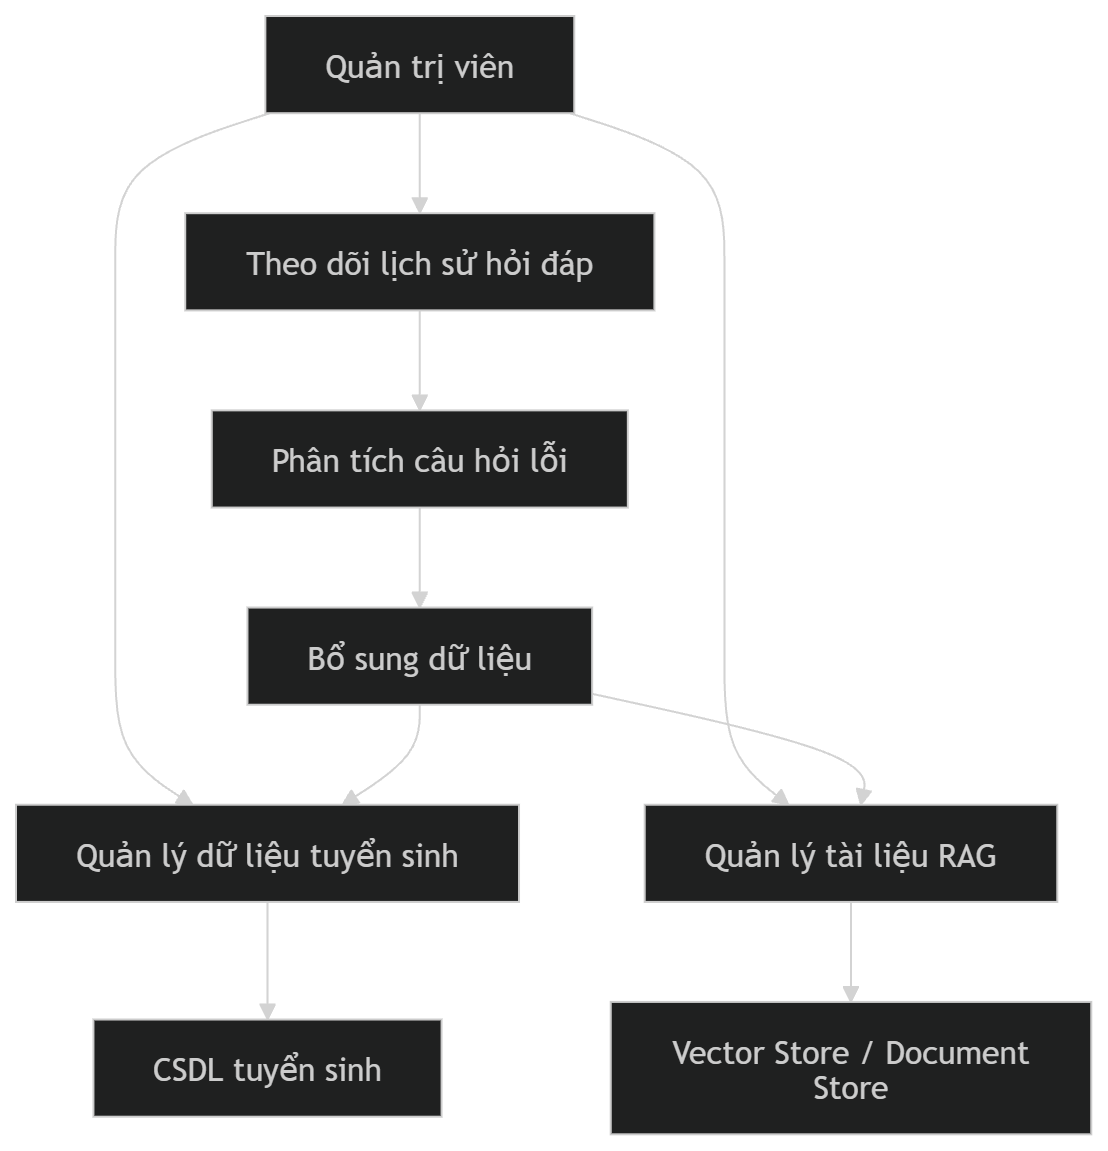
\includegraphics[width=\textwidth]{content/source/Hình 2.7 Luồng quản trị dữ liệu và cải thiện chatbot..png}
    \caption{Luồng quản trị dữ liệu và cải thiện chatbot}
    \label{fig:admin_improvement_flow}
\end{figure}
